\section{Objectives and Methodologies}
\label{sec:chromium-objectives}


\subsection{Research questions}

We start our analysis by assessing the effectiveness of the existing flakiness prediction methods in our project by considering the critical cases where fault-revealing test failures are flagged as flaky by the prediction methods in various CI cycles. We thus are interested in investigating the methods' performance under realistic settings, i.e., correctly detected and missed flaky and fault-triggering test failures, when trained with past CI data and evaluated on future ones. In contrast to previous work, this analysis introduces a new dimension in the evaluation of flakiness predictions which is the investigation of what we lose when adopting a prediction method (the fault-triggering failures classified as flaky). Therefore, we ask:

\begin{description}
\item[RQ1:] How well do flaky test prediction methods discern flaky test failures from fault-triggering ones? 
\end{description}

To establish realistic settings, we train the prediction models using the information available (flaky tests and non-flaky ones) at a given point in time, where we have sufficient historical data to train on. We then evaluate the models in subsequent builds with respect to flaky and fault-triggering test failures. 
% To avoid coincidental results, we repeat the process multiple times at different points in time, i.e., with different training and evaluation data. 
We replicate the vocabulary-based methods since they are popular, easy to implement and quite effective, and aimed at learning to predict flaky tests, as done by previous studies.

After checking the prediction performance in a realistic setting (test failures), we repeat the entire process but now we train on historical test failures instead of tests. We make this adaptation with the hope of improving further our predictions and perhaps improving our understanding of the impact that such predictions may have on missed fault-triggering test failures (those marked by the models as flaky). Hence, we ask: 

\begin{description}
\item[RQ2:] How well do flaky test failure prediction methods discern flaky test failures from fault-triggering ones? 
\end{description}

Finally, we wish to be comprehensive, so we also optimize and extend the prediction methods with additional features, some of which were suggested by previous studies (the flake rate~\cite{Kowalczyk2020}, the run duration~\cite{alshammari2021flakeflagger}) and some dynamic features (test run status, test run tag status, test run duration) that we found by us when experimenting with the flaky tests. Thus, we ask:

\begin{description}
\item[RQ3:] Can we improve the accuracy of the flaky test failure predictions by considering dynamic test execution features?
\end{description}

To answer RQ3, we repeat the analysis carried out for RQ2 but now we are training and optimising for the additional features that we determined during our analysis and check the performance we achieve with regards to test failures, as performed in RQ2. 



%With this case study, we first seek to understand the prevalence of flaky tests in the Chromium project. We are especially interested in the critical cases where regressions are reported by flaky tests. Then, we aim at contrasting two different tasks:

%\begin{itemize}
 %   \item \textbf{Objective I: Discerning flaky tests from non-flaky tests.} Broad attention is currently given by the research community towards the problem of detecting flaky tests. The motivation is the following: Flaky tests represent a major concern in software testing as they force developers to investigate false alerts and rerunning tests can be costly. Training a classifier to predict flaky tests would help focus on tests that are the most likely to be flaky first, or could be used as an alternative to reruns.
%    \item \textbf{Objective II: Discerning legitimate failures from flaky failures.}
%    Fewer studies are addressing the problem of classifying legitimate failures and flaky failures. However, our findings lead us to focus on failure detection. It is the execution of a test and its context that needs to be considered as the same test could lead to a flaky failure in one build and to a legitimate failure in another. An efficient solution to this problem has the potential of reducing rerunning costs and helping developers get better insights into their test outcomes.
%\end{itemize}


\subsection{Experimental procedure}

\subsubsection{Selection of a flaky test detection approach} 
\label{sec:evaluationSelection}
Being a recent topic of interest, several techniques have been introduced in the scientific literature. Approaches relying on code coverage such as FlakeFlagger~\cite{alshammari2021flakeflagger} or DeFlaker~\cite{Bell2018} are challenging to implement in our case. Chromium's code base consists of several languages and code coverage is both costly and non-trivial to retrieve. Test smells~\cite{camara2021use} approaches are also difficult to extract as tests are written in many different languages and tools do not always exist. 
% Another recent fully-static approach that was presented in the literature is Peeler~\cite{qin2022peeler}. Peeler's features rely on test dependency graphs that are generated using contextual paths between each test and their code under test. It was implemented in Java. Unfortunately for us, Java is not a prevalent language in Chromium's tests. 
Having those constraints in mind, we decide to use the vocabulary-based approach introduced by Pinto~\etal ~\cite{Pinto2020}. It received significant attention with several replication studies conducted~\cite{Haben2021,Camara2021VocabExtendedReplication} and follow-up studies and its portability makes it easy to implement regardless of the languages being used.

\subsubsection{Training and validation of the existing approaches (RQ1)} 
We evaluate the ability of the vocabulary-based approach, trained to differentiate flaky from non-flaky tests and used to predict flaky test failures. To do so, we divide our dataset into a training set (containing test information about the first 8,000 builds) and a test set (containing test information about the last 2,000 builds). We train our model following the existing methodologies. The flaky set includes all tests marked as flaky in the training set. 
The non-flaky set includes all fault-revealing tests and all passing tests in the 8,000\textsuperscript{th} build (\ie the last build of the training set) minus the tests that are found as flaky in any of the builds under study (to increase the confidence of being non-flaky). The test set includes all flaky test failures and all fault-triggering failures (reported by fault-revealing tests). The test set is common in all RQs.
% We discuss performances in two scenarios: the first, where we keep duplicated tests and the second, where we remove them. Usually, when evaluating a machine learning model, we remove duplicated data points to evaluate its ability to work on unseen data. In our case, a large part of the dataset consists of duplicated tests, as the same tests are executed in every build (with few additions and deletions brought by development). We believe the two scenarios are useful to report, as in a practical setup, the model would be given tests already seen in the past in most cases, but we still want to understand if feature trends can be found and used to identify unseen tests.

\subsubsection{Implementation of a failure classifier (RQ2 and RQ3)}
We select flaky failures in our dataset as all failures produced by flaky tests and fault-triggering failures are all failures produced by fault-revealing tests. There are no duplicated data in the case of test failures, as each test execution is unique. For RQ2, we train our classifier on non-flaky executions (passing and fault-revealing tests execution) and flaky failures. In RQ3, we report the performance of a model using execution features (run duration and flake rate).

\subsubsection{Time-sensitive evaluation}
We split our data in two parts: the first 80\% builds are selected as a training set and the last 20\% as a holdout set. By doing so, we respect the evolution of failures across time and avoid any data leakage that could occur by randomly selecting data. This time-sensitive aspect is very important to consider. We found that not taking this condition into account and training a model on a shuffled dataset would greatly overestimate the performance. Figure~\ref{fig:dataset} shows a representation of our dataset. Flaky tests are present in all builds and Fault-revealing tests are occasional: they happen in \nicefrac{1}{4} of builds (See Section~\ref{sec:chromium-discussion}). To mitigate imbalance, we collected all passing tests for 1 build: $b_{8,000}$ and use them in our set of non-flaky tests, for training.

% Figure dataset
\begin{figure*}[t]
\vspace{-1.4em}
\centering
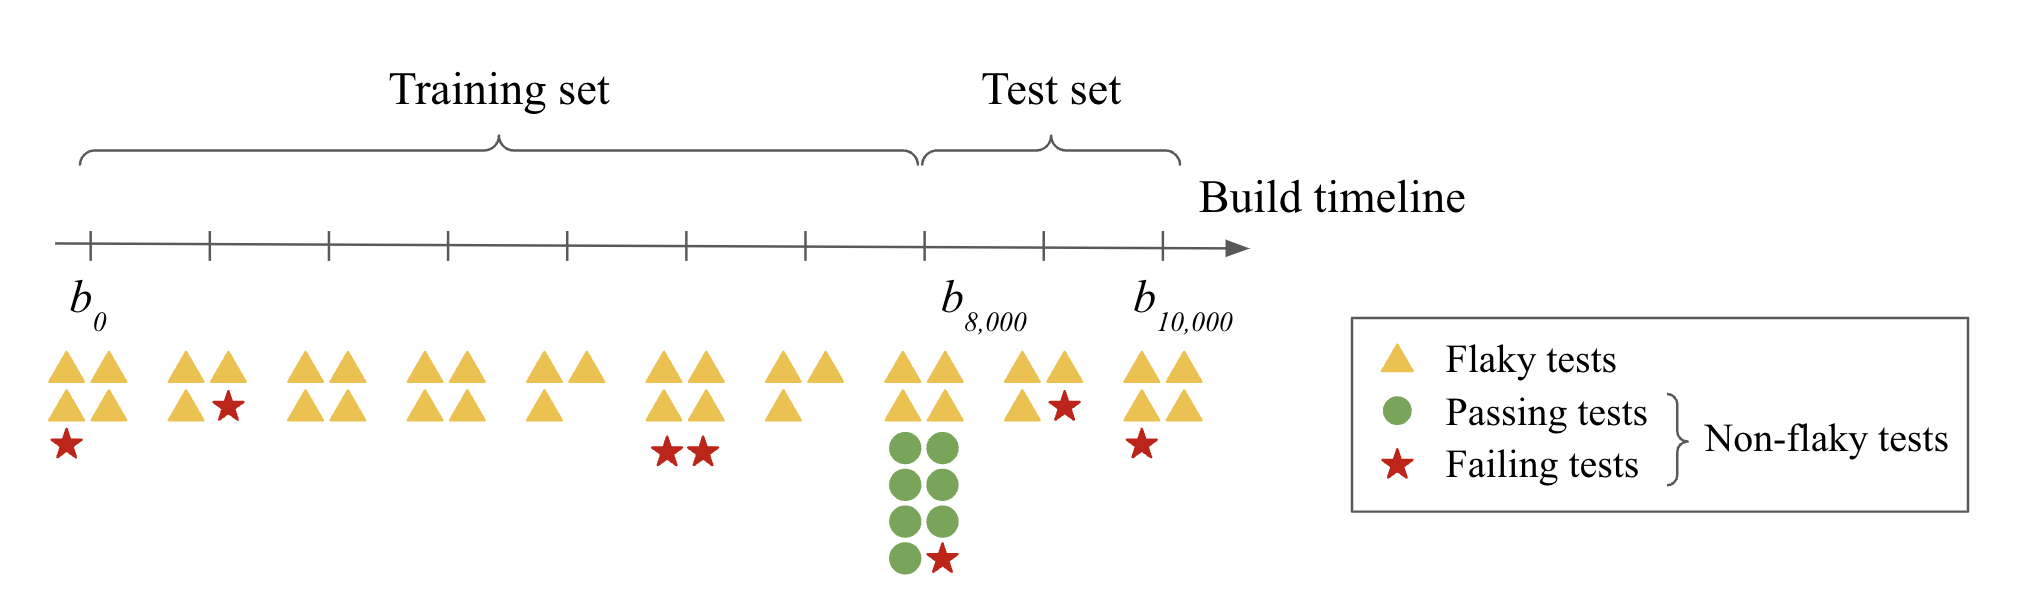
\includegraphics[width=0.8\textwidth]{figures/chromium/dataset.png}
\vspace{-1.1em}
\caption{The data collected from Chromium's CI consists of flaky, fault-revealing and passing tests spread across 10,000 builds. The build timeline ranges from build \textit{$b_0$} to \textit{$b_{10,000}$} and depicts the distribution of the collected tests: flaky tests are spread across all builds and fault-revealing tests happen occasionally. Due to a large number of passing tests, we collected them from the \textit{$b_{8,000}$} build (\ie at the end of our training set).}
\label{fig:dataset}
\vspace{-0.2em}
\end{figure*}

\subsubsection{Classifier selection and pipeline description}
% Model 
We use a random forest classifier to perform the predictions. Unfortunately, our dataset is imbalanced with the minority class being 1\% of the data. Using a simple random forest would greatly increase the chance of having few or no elements from our minority class in the different trees, making the overall model poor in predicting the class of interest. To alleviate this issue, we decide to use a Balanced Random Forest classifier\cite{chen2004using} to facilitate the learning. This implementation artificially modifies the class distribution in each tree so that they are equally represented. Furthermore, we use SMOTE in the training phase to augment data for the minority class~\cite{smote}.

% Test source representation
To represent the tests, we use \textit{CountVectorizer} to convert texts as a matrix of token counts. This technique, known as bag-of-words, is used in previous vocabulary-based approaches~\cite{Pinto2020,Haben2021,Camara2021VocabExtendedReplication,Bertolino2020,olewickiBrown}. These vectors initially contain as many features as the words appearing in source code of the tests. As the generated dictionary can become big (in terms of size) we need to use feature selection to reduce it, remove irrelevant features (reducing noise in the data) and select the most informative features. Feature selection is thus, helping to reduce the model training time and to improve the overall performance and interpretability of the model. 

We use SelectKBest\cite{selectkbest} which retains the $k$ highest score features based on the univariate statistical test $\chi^2$.
Hyper-parameters of the machine learning pipeline, \ie the number of trees in the forests, the sampling strategy for SMOTE and the number of features to be retained are tuned using a grid search approach and cross-validation in the training set. Once optimized, we retrain a model fitted on the whole training set and evaluate it on the holdout set.

\subsubsection{Metrics}
Finally, to evaluate the different models, we rely on the following metrics derived from true positives (TP), true negatives (TN), false positives (FP) and false negatives (FN):
    \[
    \textbf{Precision} = \frac{TP}{TP+FP} \quad \quad \quad \textbf{Recall} = \frac{TP}{TP+FN}
    \]
The accuracy of a model is sensitive to class imbalance. In particular, the precision and recall metrics can easily be impacted when one class is underrepresented. To alleviate this issue, we report the Matthews Correlation Coefficient (MCC) which is a more reliable statistical rate to avoid over-optimistic results in the case of an imbalanced dataset \cite{chicco2020advantages}.
This metric takes into consideration all four entries of the confusion matrix. MCC ranges from -1 to 1 and is given by the following formula: 
    \[
    \textbf{MCC} = \frac{TN \times TP - FP \times FN}{\sqrt{(TN+FN)(TP+FP)(TN+FP)(FN+TP)}}
    \]
In addition to those metrics, we also report the false positive rate (FPR), that is, the ratio of fault-triggering failures misclassified as flaky over all fault-triggering failures. It is defined by:
    \[
    \textbf{FPR} = \frac{FP}{FP+TN}
    \]
%In our case, the FPR is the proportion of fault-revealing tests incorrectly classified as flaky (\ie missed faults). The FNR is the proportion of flaky tests incorrectly classified as fault-revealing (\ie false alerts). 